\documentclass{standalone}
\usepackage{tikz}
\usetikzlibrary{patterns, positioning}


\begin{document}
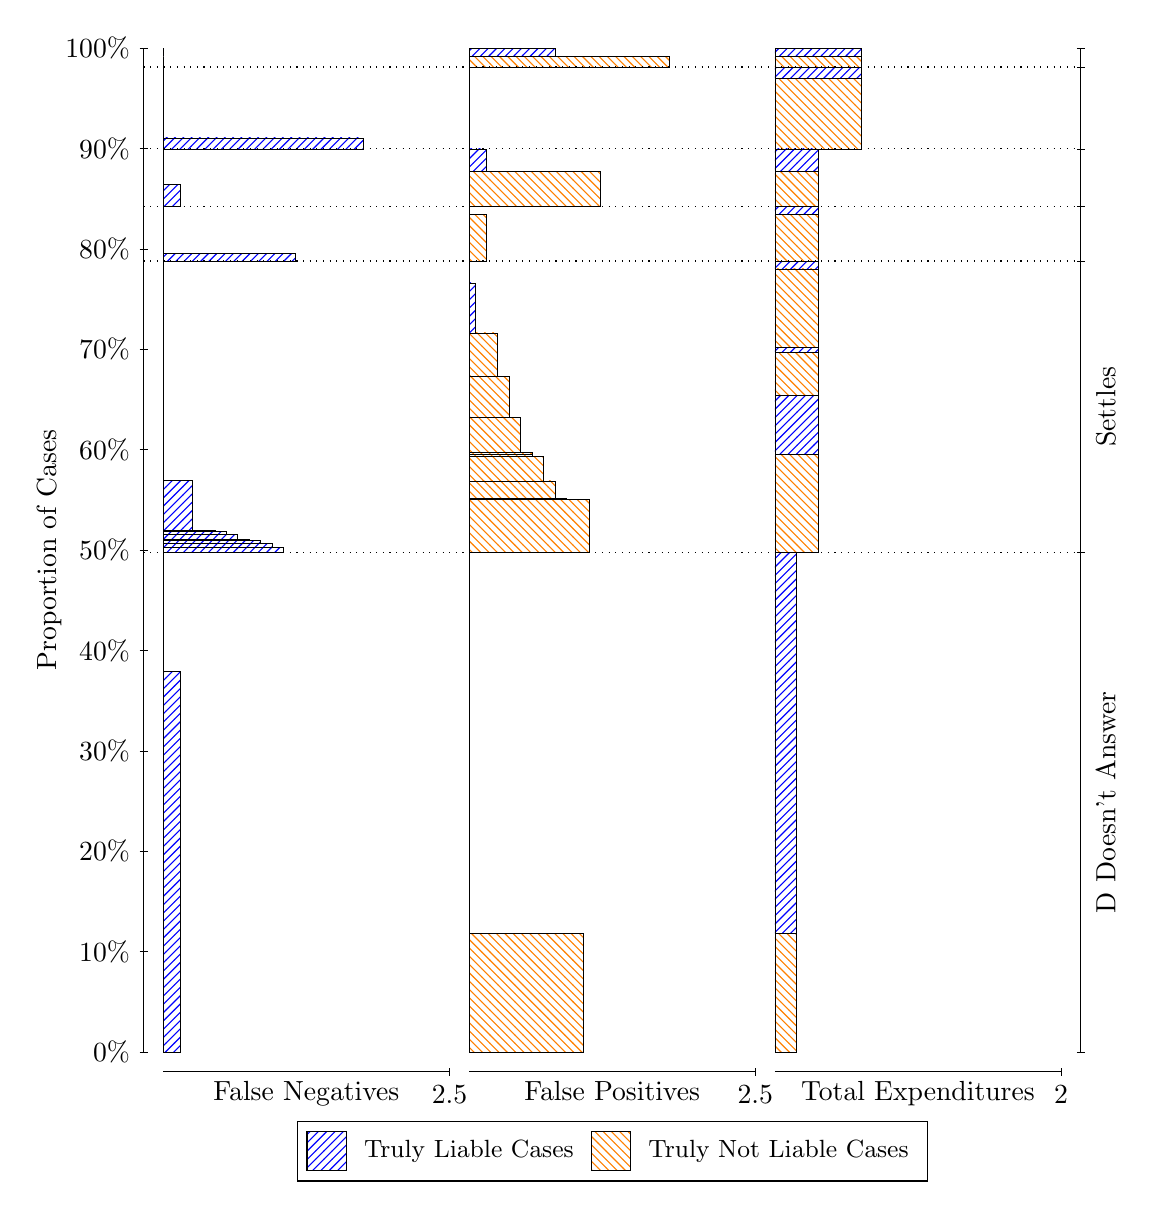
\begin{tikzpicture}
\draw[black, very thin] (1.5,1.75) -- (1.5,14.5);
\node[rotate=90, text=black, anchor=center] at (0.3, 8.125) {Proportion of Cases};
\draw[black, very thin] (1.45,1.75) -- (1.55,1.75);
\node[text=black, anchor=east] at (1.45, 1.75) {0\%};
\draw[black, very thin] (1.45,3.025) -- (1.55,3.025);
\node[text=black, anchor=east] at (1.45, 3.025) {10\%};
\draw[black, very thin] (1.45,4.3) -- (1.55,4.3);
\node[text=black, anchor=east] at (1.45, 4.3) {20\%};
\draw[black, very thin] (1.45,5.575) -- (1.55,5.575);
\node[text=black, anchor=east] at (1.45, 5.575) {30\%};
\draw[black, very thin] (1.45,6.85) -- (1.55,6.85);
\node[text=black, anchor=east] at (1.45, 6.85) {40\%};
\draw[black, very thin] (1.45,8.125) -- (1.55,8.125);
\node[text=black, anchor=east] at (1.45, 8.125) {50\%};
\draw[black, very thin] (1.45,9.4) -- (1.55,9.4);
\node[text=black, anchor=east] at (1.45, 9.4) {60\%};
\draw[black, very thin] (1.45,10.675) -- (1.55,10.675);
\node[text=black, anchor=east] at (1.45, 10.675) {70\%};
\draw[black, very thin] (1.45,11.95) -- (1.55,11.95);
\node[text=black, anchor=east] at (1.45, 11.95) {80\%};
\draw[black, very thin] (1.45,13.225) -- (1.55,13.225);
\node[text=black, anchor=east] at (1.45, 13.225) {90\%};
\draw[black, very thin] (1.45,14.5) -- (1.55,14.5);
\node[text=black, anchor=east] at (1.45, 14.5) {100\%};

\draw[black, very thin] (13.4,1.75) -- (13.4,14.5);
\draw[black, very thin] (13.35,1.75) -- (13.45,1.75);
\node[anchor=west] at (13.35, 1.75) {};
\draw[black, very thin] (13.35,8.0947) -- (13.45,8.0947);
\node[anchor=west] at (13.35, 8.0947) {};
\draw[black, very thin] (13.35,11.795) -- (13.45,11.795);
\node[anchor=west] at (13.35, 11.795) {};
\draw[black, very thin] (13.35,12.485) -- (13.45,12.485);
\node[anchor=west] at (13.35, 12.485) {};
\draw[black, very thin] (13.35,13.22) -- (13.45,13.22);
\node[anchor=west] at (13.35, 13.22) {};
\draw[black, very thin] (13.35,14.259) -- (13.45,14.259);
\node[anchor=west] at (13.35, 14.259) {};
\draw[black, very thin] (13.35,14.5) -- (13.45,14.5);
\node[anchor=west] at (13.35, 14.5) {};

\draw[black, very thin, pattern color=blue, pattern=north east lines] (1.75,1.75) rectangle (1.968,6.588);
\draw[black, very thin, pattern color=orange, pattern=north west lines] (1.75,6.588) rectangle (1.75,8.0947);
\draw[black, very thin, pattern color=blue, pattern=north east lines] (1.75,8.0947) rectangle (3.276,8.1546);
\draw[black, very thin, pattern color=blue, pattern=north east lines] (1.75,8.1546) rectangle (3.1307,8.2086);
\draw[black, very thin, pattern color=blue, pattern=north east lines] (1.75,8.2086) rectangle (2.9853,8.2519);
\draw[black, very thin, pattern color=blue, pattern=north east lines] (1.75,8.2519) rectangle (2.84,8.2589);
\draw[black, very thin, pattern color=blue, pattern=north east lines] (1.75,8.2589) rectangle (2.6947,8.3244);
\draw[black, very thin, pattern color=blue, pattern=north east lines] (1.75,8.3244) rectangle (2.5493,8.3661);
\draw[black, very thin, pattern color=blue, pattern=north east lines] (1.75,8.3661) rectangle (2.404,8.3693);
\draw[black, very thin, pattern color=blue, pattern=north east lines] (1.75,8.3693) rectangle (2.2587,8.3723);
\draw[black, very thin, pattern color=blue, pattern=north east lines] (1.75,8.3723) rectangle (2.1133,9.0066);
\draw[black, very thin, pattern color=orange, pattern=north west lines] (1.75,9.0066) rectangle (1.75,11.795);
\draw[black, very thin, pattern color=blue, pattern=north east lines] (1.75,11.795) rectangle (3.4213,11.891);
\draw[black, very thin, pattern color=orange, pattern=north west lines] (1.75,11.891) rectangle (1.75,12.485);
\draw[black, very thin, pattern color=blue, pattern=north east lines] (1.75,12.485) rectangle (1.968,12.769);
\draw[black, very thin, pattern color=orange, pattern=north west lines] (1.75,12.769) rectangle (1.75,13.22);
\draw[black, very thin, pattern color=blue, pattern=north east lines] (1.75,13.22) rectangle (4.2933,13.359);
\draw[black, very thin, pattern color=orange, pattern=north west lines] (1.75,13.359) rectangle (1.75,14.259);
\draw[black, very thin, pattern color=orange, pattern=north west lines] (1.75,14.259) rectangle (1.75,14.395);
\draw[black, very thin, pattern color=blue, pattern=north east lines] (1.75,14.395) rectangle (1.75,14.5);
\draw[black, very thin, pattern color=orange, pattern=north west lines] (5.6333,1.75) rectangle (7.0867,3.2567);
\draw[black, very thin, pattern color=blue, pattern=north east lines] (5.6333,3.2567) rectangle (5.6333,8.0947);
\draw[black, very thin, pattern color=orange, pattern=north west lines] (5.6333,8.0947) rectangle (7.1593,8.7675);
\draw[black, very thin, pattern color=orange, pattern=north west lines] (5.6333,8.7675) rectangle (7.014,8.7716);
\draw[black, very thin, pattern color=orange, pattern=north west lines] (5.6333,8.7716) rectangle (6.8687,8.776);
\draw[black, very thin, pattern color=orange, pattern=north west lines] (5.6333,8.776) rectangle (6.7233,9.002);
\draw[black, very thin, pattern color=orange, pattern=north west lines] (5.6333,9.002) rectangle (6.578,9.3155);
\draw[black, very thin, pattern color=orange, pattern=north west lines] (5.6333,9.3155) rectangle (6.4327,9.3344);
\draw[black, very thin, pattern color=orange, pattern=north west lines] (5.6333,9.3344) rectangle (6.4327,9.3607);
\draw[black, very thin, pattern color=orange, pattern=north west lines] (5.6333,9.3607) rectangle (6.2873,9.8094);
\draw[black, very thin, pattern color=orange, pattern=north west lines] (5.6333,9.8094) rectangle (6.142,10.334);
\draw[black, very thin, pattern color=orange, pattern=north west lines] (5.6333,10.334) rectangle (5.9967,10.883);
\draw[black, very thin, pattern color=blue, pattern=north east lines] (5.6333,10.883) rectangle (5.706,11.518);
\draw[black, very thin, pattern color=blue, pattern=north east lines] (5.6333,11.518) rectangle (5.6333,11.795);
\draw[black, very thin, pattern color=orange, pattern=north west lines] (5.6333,11.795) rectangle (5.8513,12.389);
\draw[black, very thin, pattern color=blue, pattern=north east lines] (5.6333,12.389) rectangle (5.6333,12.485);
\draw[black, very thin, pattern color=orange, pattern=north west lines] (5.6333,12.485) rectangle (7.3047,12.936);
\draw[black, very thin, pattern color=blue, pattern=north east lines] (5.6333,12.936) rectangle (5.8513,13.22);
\draw[black, very thin, pattern color=orange, pattern=north west lines] (5.6333,13.22) rectangle (5.6333,14.119);
\draw[black, very thin, pattern color=blue, pattern=north east lines] (5.6333,14.119) rectangle (5.6333,14.259);
\draw[black, very thin, pattern color=orange, pattern=north west lines] (5.6333,14.259) rectangle (8.1767,14.395);
\draw[black, very thin, pattern color=blue, pattern=north east lines] (5.6333,14.395) rectangle (6.7233,14.5);
\draw[black, very thin, pattern color=orange, pattern=north west lines] (9.5167,1.75) rectangle (9.7892,3.2567);
\draw[black, very thin, pattern color=blue, pattern=north east lines] (9.5167,3.2567) rectangle (9.7892,8.0947);
\draw[black, very thin, pattern color=orange, pattern=north west lines] (9.5167,8.0947) rectangle (10.062,9.3344);
\draw[black, very thin, pattern color=blue, pattern=north east lines] (9.5167,9.3344) rectangle (10.062,10.085);
\draw[black, very thin, pattern color=orange, pattern=north west lines] (9.5167,10.085) rectangle (10.062,10.634);
\draw[black, very thin, pattern color=blue, pattern=north east lines] (9.5167,10.634) rectangle (10.062,10.694);
\draw[black, very thin, pattern color=orange, pattern=north west lines] (9.5167,10.694) rectangle (10.062,11.694);
\draw[black, very thin, pattern color=blue, pattern=north east lines] (9.5167,11.694) rectangle (10.062,11.795);
\draw[black, very thin, pattern color=orange, pattern=north west lines] (9.5167,11.795) rectangle (10.062,12.389);
\draw[black, very thin, pattern color=blue, pattern=north east lines] (9.5167,12.389) rectangle (10.062,12.485);
\draw[black, very thin, pattern color=orange, pattern=north west lines] (9.5167,12.485) rectangle (10.062,12.936);
\draw[black, very thin, pattern color=blue, pattern=north east lines] (9.5167,12.936) rectangle (10.062,13.22);
\draw[black, very thin, pattern color=orange, pattern=north west lines] (9.5167,13.22) rectangle (10.607,14.119);
\draw[black, very thin, pattern color=blue, pattern=north east lines] (9.5167,14.119) rectangle (10.607,14.259);
\draw[black, very thin, pattern color=orange, pattern=north west lines] (9.5167,14.259) rectangle (10.607,14.395);
\draw[black, very thin, pattern color=blue, pattern=north east lines] (9.5167,14.395) rectangle (10.607,14.5);
\draw[black, dotted] (1.5,8.0947) -- (13.4,8.0947);
\draw[black, dotted] (1.5,11.795) -- (13.4,11.795);
\draw[black, dotted] (1.5,12.485) -- (13.4,12.485);
\draw[black, dotted] (1.5,13.22) -- (13.4,13.22);
\draw[black, dotted] (1.5,14.259) -- (13.4,14.259);
\draw[black, very thin] (1.75,1.5) -- (5.3833,1.5);
\node[text=black, anchor=north] at (3.5667, 1.5) {False Negatives};
\draw[black, very thin] (5.3833,1.45) -- (5.3833,1.55);
\node[text=black, anchor=north] at (5.3833, 1.45) {2.5};

\draw[black, very thin] (5.6333,1.5) -- (9.2667,1.5);
\node[text=black, anchor=north] at (7.45, 1.5) {False Positives};
\draw[black, very thin] (9.2667,1.45) -- (9.2667,1.55);
\node[text=black, anchor=north] at (9.2667, 1.45) {2.5};

\draw[black, very thin] (9.5167,1.5) -- (13.15,1.5);
\node[text=black, anchor=north] at (11.333, 1.5) {Total Expenditures};
\draw[black, very thin] (13.15,1.45) -- (13.15,1.55);
\node[text=black, anchor=north] at (13.15, 1.45) {2};

\node[text=black, centered, rotate=90] at (13.72, 4.9223) {D Doesn't Answer};
\node[text=black, centered, rotate=90] at (13.72, 9.945) {Settles};





\draw (7.449999999999999,1.5) node[draw=none] (baseCoordinate) {};
\begin{scope}[align=center]
        \matrix[scale=0.5, draw=black, below=0.5cm of baseCoordinate, nodes={draw}, column sep=0.1cm]{
            \node[rectangle, draw, minimum width=0.5cm, minimum height=0.5cm, pattern color=blue, pattern=north east lines] {}; &
            \node[draw=none, font=\small, text=black] (B) {Truly Liable Cases}; &
            \node[rectangle, draw, minimum width=0.5cm, minimum height=0.5cm, pattern color=orange, pattern=north west lines] {}; &
            \node[draw=none, font=\small, text=black] (B) {Truly Not Liable Cases}; \\
            };
\end{scope}

\end{tikzpicture}
\end{document}